\section{Auswertung}
Die zu dem verwendeten Gerät gehörigen Daten lauten:
\begin{equation*}
\begin{aligned}
L   &= (10{,}11 \pm 0{,}03)\cdot 10^{-3}\,\symup{H} \\
C   &= (2{,}098 \pm 0{,}006)\cdot 10^{-9}\, \symup{F} \\
R_1 &= (48{,}1   \pm 0{,}1)   \, \symup{\Omega} \\
R_2 &= (509{,}5  \pm 0{,}5)   \, \symup{\Omega}
\end{aligned}
\end{equation*}

\subsection{Berechnung der Abklingdauer und des effektiven Widerstands}

\begin{figure}[h!]
	\centering
	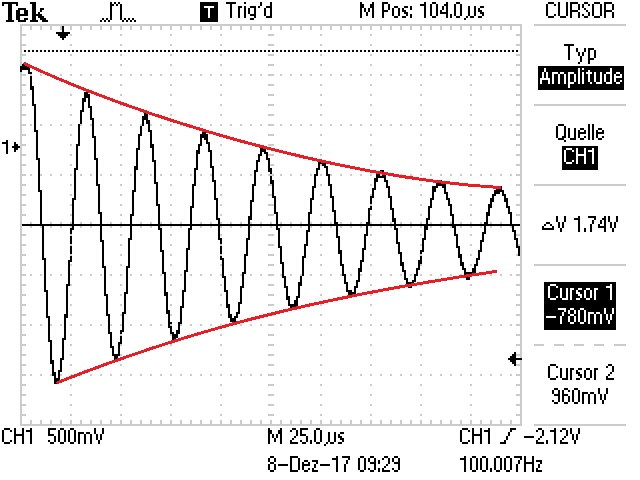
\includegraphics[width=0.7\linewidth]{Einhuellende.jpg}
	\caption{Thermodruck des Abklingvorgangs.}
	\label{fig:thermodruck}
\end{figure}

Abbildung \eqref{fig:thermodruck} zeigt den Thermodruck der gedämpften Schwingung der Kondensatorspannung $U_{\text{C}}$ mit eingezeichneter Einhüllende.
Diese Hülle kann durch die Funktion

\begin{equation}
A=A_0 \cdot e^{-2\pi \mu t}
\label{eq:Ausgleichskurve}
\end{equation}
beschrieben werden. Zur Berechnung von $A_0$ und $\mu$ werden die gemessenen Spannungsamplituden $U_{\text{C}}$ und Zeiten $t$, welche in Tabelle \eqref{tab:spannungundzeit} zu finden sind, gegeneinander aufgetragen.
\begin{table}[h!]
   \centering
   \caption{Messdaten von Spannung und Zeit zur Bestimmung der Abklingdauer und des effektiven Dämpfungswiderstandes.}
   \label{tab:spannungundzeit}
   \begin{tabular}{
S[table-format=1.2, table-auto-round] 
S[table-format=3.0, table-auto-round]
}
\toprule
{$U_{\text{C}}/\,\symup{V}$} & {$t/10^{-6}\,\symup{s}$} \\
\midrule
1.6  & -21 \\
1.54 & -3  \\
1.3  & 11 \\
1.3  & 26 \\
1.1  & 41 \\
1.1  & 56 \\
0.94 & 70 \\
0.92 & 85 \\
0.82 & 100 \\
0.82 & 115 \\
0.68 & 130 \\
0.68 & 144 \\
0.56 & 159 \\
0.58 & 174 \\
0.46 & 189 \\
\bottomrule
\end{tabular}
\end{table}

\begin{figure}[h!]
	\centering
	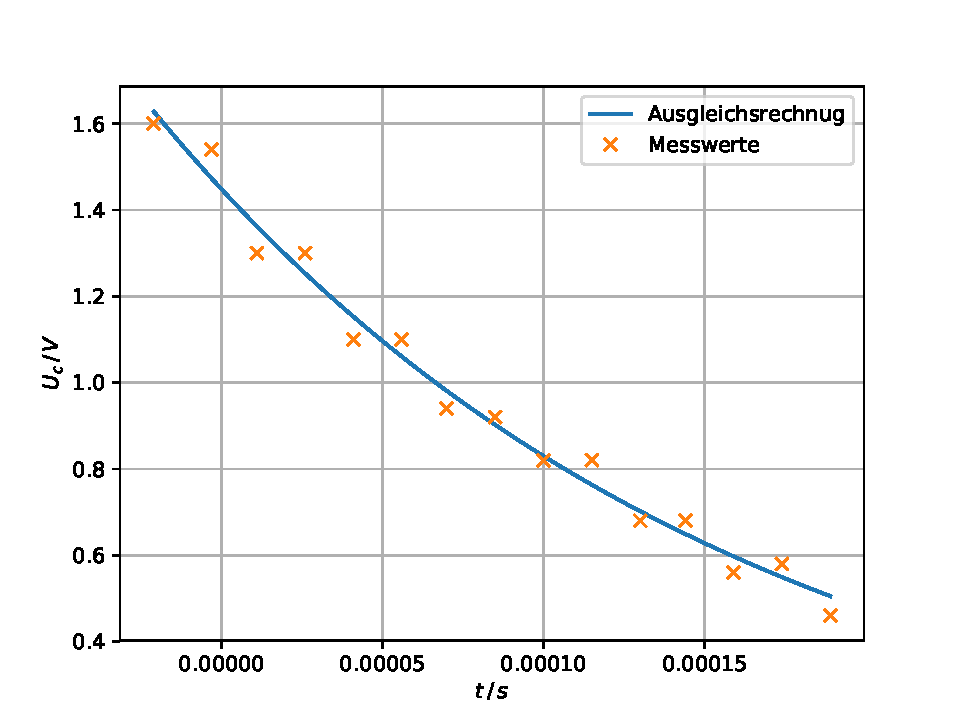
\includegraphics[width=0.7\linewidth]{test.pdf}
	\caption{Exponentielle Regression der Spannungsamplituden.}
	\label{fig:spannungregression}
\end{figure}
Mit dem Python-Modul Matplotlib wird eine exponentielle Ausgleichskurve der Form von Gleichung \eqref{eq:Ausgleichskurve} erstellt. Daraus ergibt sich:
\begin{equation*}
\begin{aligned}
A_0 &= (1{,}4481 \pm 0{,}0004)\, \symup{V} \\
\mu &= (886{,}8 \pm 1071{,}5)\, \symup{\frac{1}{s}}.
\end{aligned}
\end{equation*}

Nach Umstellen von Gleichung \eqref{eq:Fallunterscheidung} nach $R=R_{\text{eff}}$ kann der Effektivwiderstand berechnet werden. Da hierbei $L$ und $\mu$ fehlerbehaftete Größen sind, wird der Fehler
$\Delta R_{\text{eff}}$ mithife der Gaußschen Fehlerfortpflanzung berechnet:
\begin{equation*}
\begin{aligned}
\Delta R_{\text{eff}} &= \sqrt{\biggl(\frac{\partial R}{\partial L}\biggr)^2 \cdot (\Delta L)^2 + \biggl(\frac{\partial R}{\partial \mu}\biggr)^2 \cdot (\Delta \mu)^2} \\
\iff \Delta R_{\text{eff}} &= \sqrt{(4\pi \mu)^2 \cdot (\Delta L)^2 + (4\pi L)^2 \cdot (\Delta \mu)^2}.
\end{aligned}
\end{equation*}
Der Effektivwiderstand ist somit:
\begin{equation*}
R_{\text{eff}} = (112{,}66 \pm 136{,}13)\,\symup{\Omega}.
\end{equation*}

Nun wird die Abklingdauer $T_{\text{ex}}$ berechnet. Die Berechnung des experimentellen Werts erfolgt durch Nutzung des ersten Teils der Gleichung \eqref{eq:Abklingdauer} und dem bereits ermitteltem $\mu$. 
Der Fehler wird wiederum mit der Gaußschen Fehlerfortpflanzung berechnet:
\begin{equation*}
\begin{aligned}
\Delta T_{\text{ex,exp}} &= \sqrt{\biggl(\frac{\partial T_{\text{ex}}}{\partial \mu}\biggr)^2 \cdot (\Delta \mu )^2} \\
\iff \Delta T_{\text{ex,exp}} &= \sqrt{\biggl(-\frac{1}{2\pi \mu^2}\biggr)^2 \cdot (\Delta \mu )^2}.
\end{aligned}
\end{equation*}
Es ergibt sich:
\begin{equation*}
T_{\text{ex,exp}} = (1{,}79 \pm 2{,}17)\cdot 10^{-4}\, \symup{s}.
\end{equation*}

Der theoretische Wert wird mit dem zweiten Teil von Gleichung \eqref{eq:Abklingdauer}, sowie $R_1$ und $L$ ausgerechnet. Der Fehler ergibt sich mit
\begin{equation*}
\begin{aligned}
\Delta T_{\text{ex,theo}} &= \sqrt{\biggl(\frac{\partial T_{\text{ex}}}{\partial L}\biggr)^2 \cdot (\Delta L )^2 + \biggl(\frac{\partial T_{\text{ex}}}{\partial R_1}\biggr)^2 \cdot (\Delta R_1 )^2} \\
\iff \Delta T_{\text{ex,theo}} &= \sqrt{\biggl(\frac{2}{R_1}\biggr)^2 \cdot (\Delta L )^2 + \biggl(-\frac{2L}{R_1^2}\biggr)^2 \cdot (\Delta R_1 )^2}.
\end{aligned}
\end{equation*}
$T_{\text{ex,theo}}$ beträgt damit
\begin{equation*}
T_{\text{ex,theo}} = (4{,}204 \pm 0{,}015)\cdot 10^{-4}\, \symup{s}.
\end{equation*}
Die Abweichung beträgt $-57{,}4\%$.

%----------------------------------------------------------------------------------

\subsection{Bestimmung des Widerstands beim aperiodischen Grenzfall}

Der experimentell bestimmte Wert des Widerstands $R_{\text{ap}}$, bei dem der aperiodische Grenzfall eintritt, beträgt:
\begin{equation*}
R_{\text{ap,exp}} = 3{,}5 \cdot 10^{3}\, \symup{\Omega}.
\end{equation*}
Dies wird mit dem theoretischen Wert verglichen, welcher mit Gleichung \eqref{eq:widerstandap} berechnet wird. Der Fehler wird mit
\begin{equation*}
\begin{aligned}
\Delta R_{\text{ap}} &= \sqrt{\biggl(\frac{\partial R_{\text{ap}}}{\partial L}\biggr)^2 \cdot (\Delta L)^2 + \biggl(\frac{\partial R_{\text{ap}}}{\partial L}\biggr)^2 \cdot (\Delta L)^2} \\
\iff \Delta R_{\text{ap}} &= \sqrt{\biggl(\frac{1}{C\sqrt{\frac{L}{C}}}\biggr)^2 \cdot (\Delta L)^2 + \biggl(-\frac{L}{\sqrt{\frac{L}{C}}C^2}\biggr)^2 \cdot (\Delta L)^2}
\end{aligned}
\end{equation*}
berechnet. Nach Einsetzen der Werte beläuft sich $R_{\text{ap,theo}}$ auf:
\begin{equation*}
R_{\text{ap,theo}} = (4{,}39 \pm 0{,}009)\cdot 10^{3}\, \symup{\Omega}.
\end{equation*}
Es lässt sich eine Abweichung von $-20{,}3\%$ feststellen.

%----------------------------------------------------------------------------------

\subsection{Bestimmung der Frequenzabhängigkeit der Kondensatorspannung}

Die gemessene Generatorspannung beträgt:
\begin{equation*}
U_0 = 764\cdot 10^{-3}\, \symup{V}.
\end{equation*}
Zur Bestimmung der Frequenzabhängigkeit der Kondensatorspannung werden die Quotienten $\frac{U_{\text{C}}}{U_0}$ und die jeweils eingestellten Frequenzen aus Tabelle \eqref{tab:frequenzkondensatorspannung} einmal 
halblogarithmisch und einmal linear gegeneinander aufgetragen, zu sehen in den Abbildungen \eqref{fig:resonanzkurve_loga} und \eqref{fig:resonanzkurve_linear}.

\begin{table}[h!]
   \centering
   \caption{Messdaten zur Bestimmung der Frequenzabhängigkeit der Kondensatorspannung.}
   \label{tab:frequenzkondensatorspannung}
   \begin{tabular}{
S[table-format=1, table-auto-round] 
S[table-format=1.2, table-auto-round]
S[table-format=1.3, table-auto-round]
}
\toprule
{$\nu /10^{3}\,\symup{Hz}$} & {$U_{\text{C}}/\,\symup{V}$} & {$\frac{U_{\text{C}}}{U_0}$} \\
\midrule
15 & 0.93 & 1.217 \\
20 & 1.13 & 1.479 \\
25 & 1.51 & 1.976 \\
30 & 2.36 & 3.089 \\
31 & 2.6 & 3.403 \\
32 & 2.78 & 3.639 \\
33 & 2.88 & 3.769\\
34 & 2.84 & 3.717\\
35 & 2.66 & 3.482\\
36 & 2.46 & 3.219\\
37 & 2.16 & 2.827\\
38 & 1.94 & 2.539\\
39 & 1.7 & 2.225\\
40 & 1.48 & 1.937\\
45 & 0.89 & 1.165\\
50 & 0.6 & 0.785\\
55 & 0.44 & 0.576\\
60 & 0.34 & 0.445\\
\bottomrule
\end{tabular}
\end{table}
\begin{figure}[h!]
	\centering
	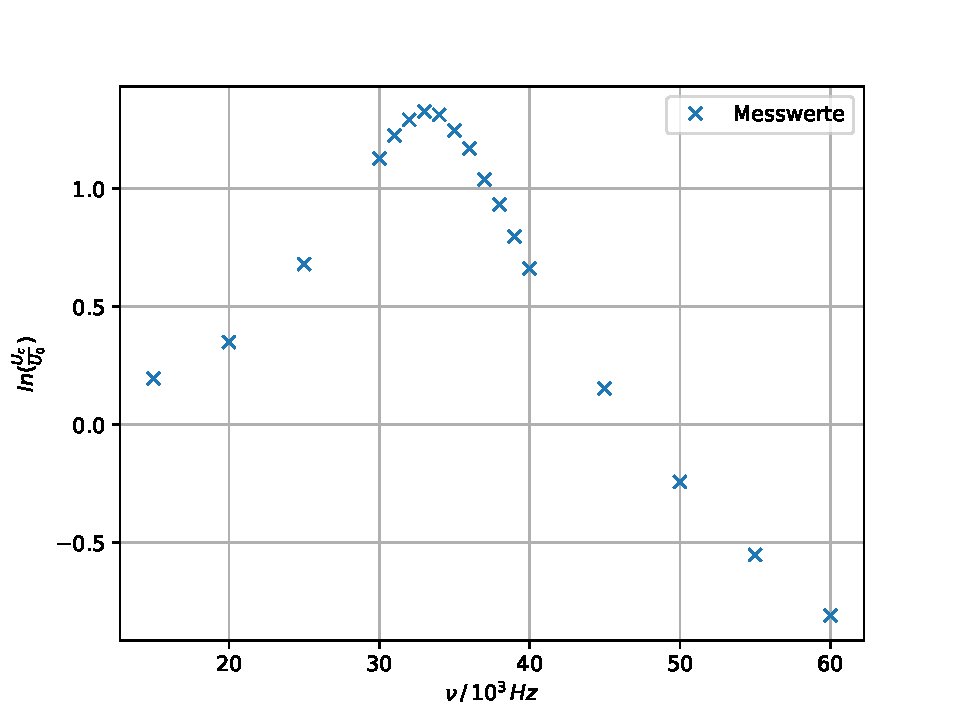
\includegraphics[width=0.8\linewidth]{FrequenzSpannung_loga.pdf}
	\caption{Halblogarithmische Darstellung der Resonanzkurve.}
	\label{fig:resonanzkurve_loga}
\end{figure}
\begin{figure}[h!]
	\centering
	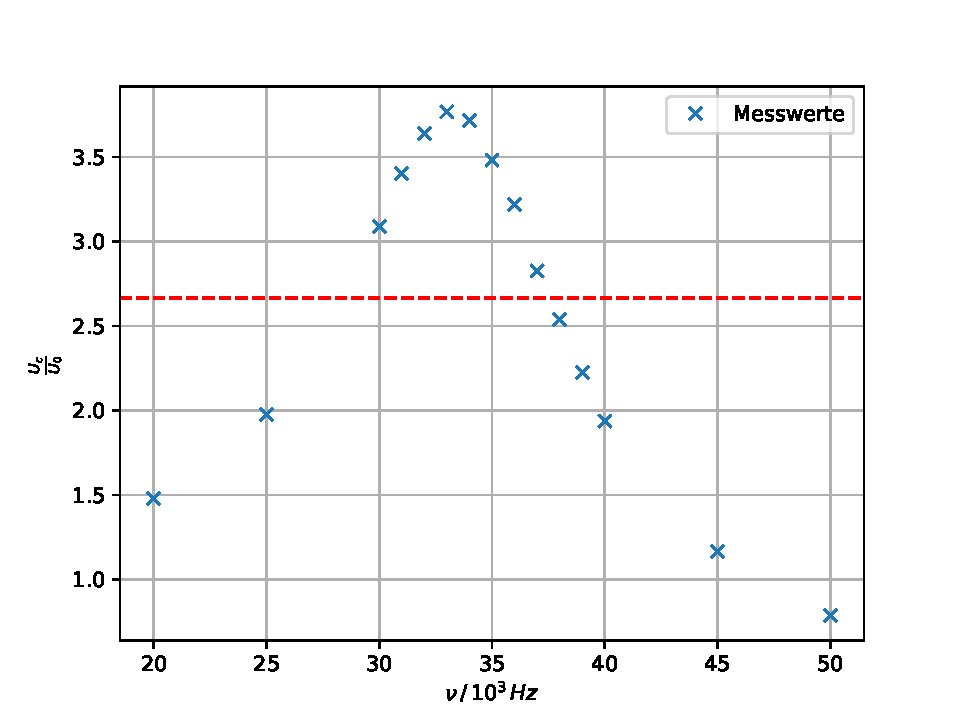
\includegraphics[width=0.7\linewidth]{FrequenzSpannung_linear.pdf}
	\caption{Lineare Darstellung der Resonanzkurve.}
	\label{fig:resonanzkurve_linear}
\end{figure}

Aus Abbildung \eqref{fig:resonanzkurve_loga} lässt sich eine Güte $q_{\text{exp}}$ von
\begin{equation*}
q_{\text{exp}} = 1{,}327
\end{equation*} 
ablesen. Der theoretische Wert der Güte wird mit Gleichung \eqref{eqn:guete} berechnet. Der Fehler $\Delta q$ ergibt sich aus:
\begin{equation*}
\begin{aligned}
\Delta q &= \sqrt{\biggl(\frac{\partial q}{\partial L}\biggr)^2\cdot (\Delta L)^2 + \biggl(\frac{\partial q}{\partial C}\biggr)^2\cdot (\Delta C)^2 + \biggl(\frac{\partial q}{\partial R}\biggr)^2\cdot (\Delta R)^2} \\
\Delta q &= \sqrt{\biggl(\frac{1}{2R\sqrt{LC}}\biggr)^2\cdot (\Delta L)^2 + \biggl(-\frac{L}{2RC\sqrt{LC}}\biggr)^2\cdot (\Delta C)^2 + \biggl(-\frac{\sqrt{LC}}{CR^2}\biggr)^2\cdot (\Delta R)^2}.
\end{aligned}
\end{equation*}
Der theoretische Wert der Güte beträgt hiermit:
\begin{equation*}
q = 4{,}309 \pm 0{,}009.
\end{equation*}
Es besteht eine Abweichung von $-69{,}2\%$.

Die Breite $(\nu_+ - \nu_-)_{\text{exp}}$ der Resonanzkurve kann aus der linearen Darstellung \eqref{fig:resonanzkurve_linear} abgelesen werden. Sie beträgt:
\begin{equation*}
(\nu_+ - \nu_-)_{\text{exp}} = 9{,}5 \cdot 10^{3}\, \symup{Hz}.
\end{equation*}
Der theoretische Wert kann über Gleichung \eqref{eq:kurvebreite} erhalten werden. Die Fehlerrechnung erfolgt mit:
\begin{equation*}
\begin{aligned}
\Delta (\nu_+ - \nu_-)_{\text{theo}} &= \sqrt{\biggl(\frac{\partial (\nu_+ - \nu_-)}{\partial R_2}\biggr)^2\cdot (\Delta R_2)^2 + \biggl(\frac{\partial (\nu_+ - \nu_-)}{\partial L}\biggr)^2\cdot (\Delta L)^2}\\
\iff \Delta (\nu_+ - \nu_-)_{\text{theo}} &= \sqrt{\biggl(\frac{1}{L}\biggr)^2\cdot (\Delta R_2)^2 + \biggl(-\frac{R_2}{L^2}\biggr)^2\cdot (\Delta L)^2}
\end{aligned}
\end{equation*}
Es ergibt sich:
\begin{equation*}
(\nu_+ - \nu_-)_{\text{theo}} = (50{,}39 \pm 0{,}16) \cdot 10^{3}\, \symup{Hz}.
\end{equation*}
Die Abweichung beträgt damit $-81{,}1 \%$.
%----------------------------------------------------------------------------------
\newpage
\subsection{Bestimmung der Frequenzabhängigkeit der Phasenverschiebung}

Die Messwerte aus Tabelle \eqref{tab:frequenzphase} sind in den Abbildungen \eqref{fig:phasenverschiebunghalbloga} und \eqref{fig:phasenverschiebunglinear} halblogarithmisch bzw. linear gegeneinander aufgetragen.

\begin{table}[h!]
   \centering
   \caption{Messdaten zur Bestimmung der Frequenzabhängigkeit der Phasenverschiebung.}
   \label{tab:frequenzphase}
   \begin{tabular}{
S[table-format=1, table-auto-round] 
S[table-format=1.2, table-auto-round]
S[table-format=1.3, table-auto-round]
}
\toprule
{$\nu /10^{3}\,\symup{Hz}$} & {$a/10^{-6}\,\symup{s}$} & {$\varphi/\,\symup{rad}$} \\
\midrule
15 & 3.2 & 0.302 \\
20 & 1.8 & 0.226 \\
25 & 2.2 & 0.346 \\
30 & 4.11 & 0.773 \\
31 & 5.0   & 0.974 \\
32 & 5.8 & 1.166 \\
33 & 6.6 & 1.368\\
34 & 7.6 & 1.624\\
35 & 8.4 & 1.847\\
36 & 8.0 & 1.809\\
37 & 9.4 & 2.185\\
38 & 9.8 & 2.339\\
39 & 10.0  & 2.450\\
40 & 10.0  & 2.513\\
45 & 9.6 & 2.714\\
50 & 9.2 & 2.890\\
55 & 8.6 & 2.972\\
60 & 7.6 & 2.865\\
\bottomrule
\end{tabular}
\end{table}
\begin{figure}[h!]
	\centering
	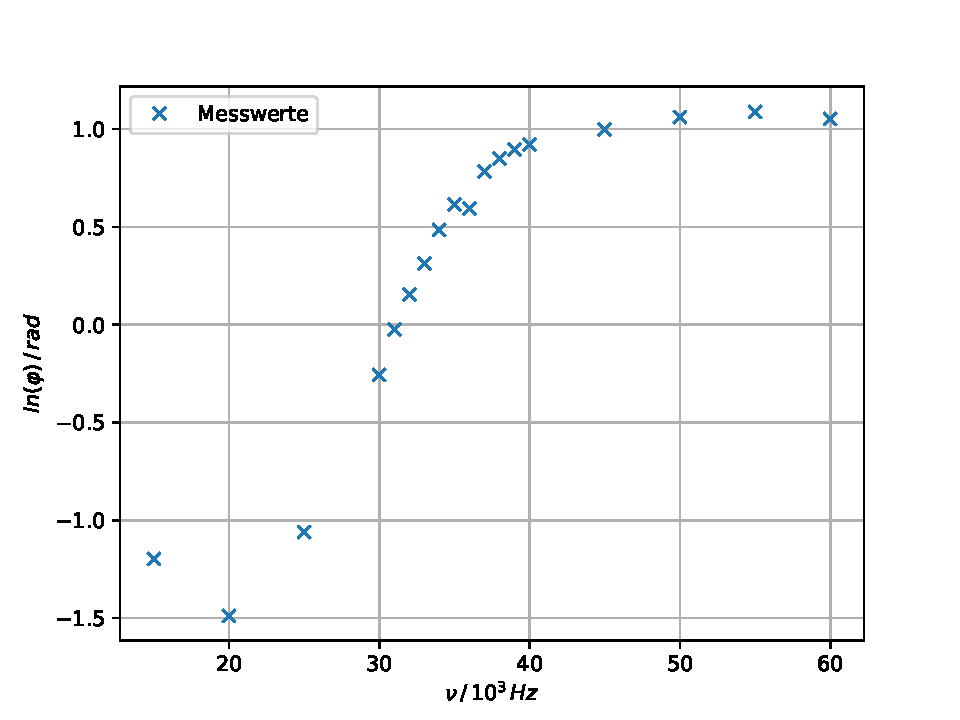
\includegraphics[width=0.7\linewidth]{phasenverschiebung2.pdf}
	\caption{Halblogarithmische Darstellung der Phasenverschiebung.}
	\label{fig:phasenverschiebunghalbloga}
\end{figure}

\begin{figure}[h!]
	\centering
	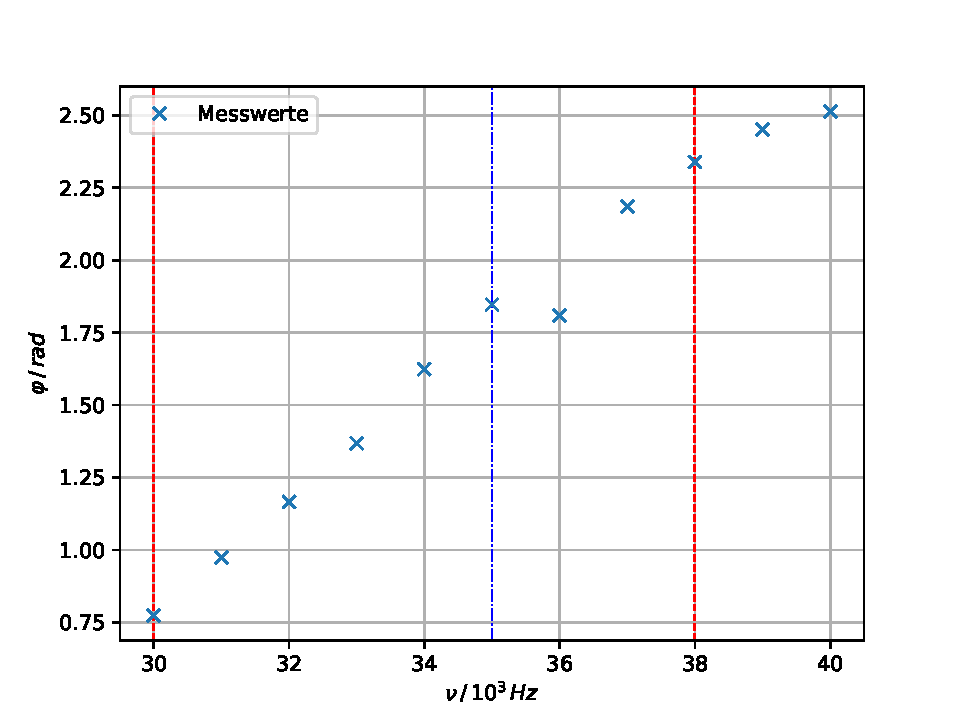
\includegraphics[width=0.7\linewidth]{phasenverschiebung.pdf}
	\caption{Lineare Darstellung der Phasenverschiebung.}
	\label{fig:phasenverschiebunglinear}
\end{figure}
Aus der linearen Darstellung lassen sich die Frequenzen $\nu_1$ und $\nu_2$ sowie die Resonanzfrequenz $\nu_{\text{res}}$ ablesen. Diese Werte werden mit den theoretischen Werten, die mit Gleichung \eqref{eq:frequenzen12}
und \eqref{eq:resonanzfrequenz} berechnet werden können, verglichen. 

\begin{equation*}
\begin{aligned} 
\nu_{\text{res,exp}} =& \, 35\,\symup{kHz} \\
\nu_{\text{res,theo}} =& \, 34{,}1\,\symup{kHz} \\
            \symup{Abweichung}:& \,  2{,}3\% \\
\nu_{\text{1,exp}} =& \, 30\,\symup{kHz} \\
\nu_{\text{1,theo}} =& \, (33{,}88 \pm 5{,}02)\,\symup{kHz}\\
\symup{Abweichung}:& \, -11{,}5\%\\
\nu_{\text{2,exp}} =& \, 38\,\symup{kHz} \\
\nu_{\text{2,theo}} =& \ (34{,}4 \pm 5{,}3)\,\symup{kHz}\\
\symup{Abweichung}:& \, 10{,}5\%\\
\end{aligned}
\end{equation*}